%%%%%%%%%%%%%%%%%%%%%%%%%%%%%%%%%%%%%%%%%%%%%%%%%%%%%%%%%%%%%%%%%%%%%%%%%%%%%%%%
\chapter{System Integration}
\label{chap:integration}

%%%%%%%%%%%%%%%%%%%%%%%%%%%%%%%%%%%%%%%%%%%%%%%%%%%%%%%%%%%%%%%%%%%%%%%%%%%%%%%%
\section{Introduction}

The RANPilotAI platform represents the integration of the intelligent software modules developed throughout this project into a unified engineering environment for Radio Access Network (RAN) optimization. Instead of operating as independent applications, the developed modules are deployed within a single web-based platform that provides centralized navigation, shared software services, and a consistent graphical user interface.

The integrated platform enables RF engineers to perform multiple optimization tasks through a common environment. Network performance can be analyzed, future KPI behaviour can be predicted, optimization recommendations can be obtained, and official 3GPP Technical Specifications can be consulted without leaving the platform. This unified workflow improves engineering productivity while reducing the complexity associated with switching between multiple software tools.

From a software engineering perspective, the platform follows a modular architecture in which each analytical module encapsulates its own processing logic while sharing common infrastructure services. This design simplifies maintenance, improves scalability, and allows future analytical modules to be integrated with minimal architectural modifications.

This chapter describes the integration architecture adopted in the RANPilotAI platform, presents the overall organization of the developed modules, and explains the software engineering principles that guided the implementation of the integrated system.

%%%%%%%%%%%%%%%%%%%%%%%%%%%%%%%%%%%%%%%%%%%%%%%%%%%%%%%%%%%%%%%%%%%%%%%%%%%%%%%%
\section{Overall Platform Architecture}

The RANPilotAI platform adopts a modular architecture in which the Telecom Hub functions as the central access point to all developed analytical modules. Rather than interacting directly with the individual processing engines, users communicate exclusively with the Telecom Hub, which manages application routing, session handling, and interaction with the underlying analytical components.

Figure~\ref{fig:platform_architecture} illustrates the overall architecture of the integrated platform.

%%%%%%%%%%%%%%%%%%%%%%%%%%%%%%%%%%%%%%%%%%%%%%%%%%%%%%%%%%%%%%%%%%%%%%%%%%%%%%%%

\begin{figure}[H]
\centering

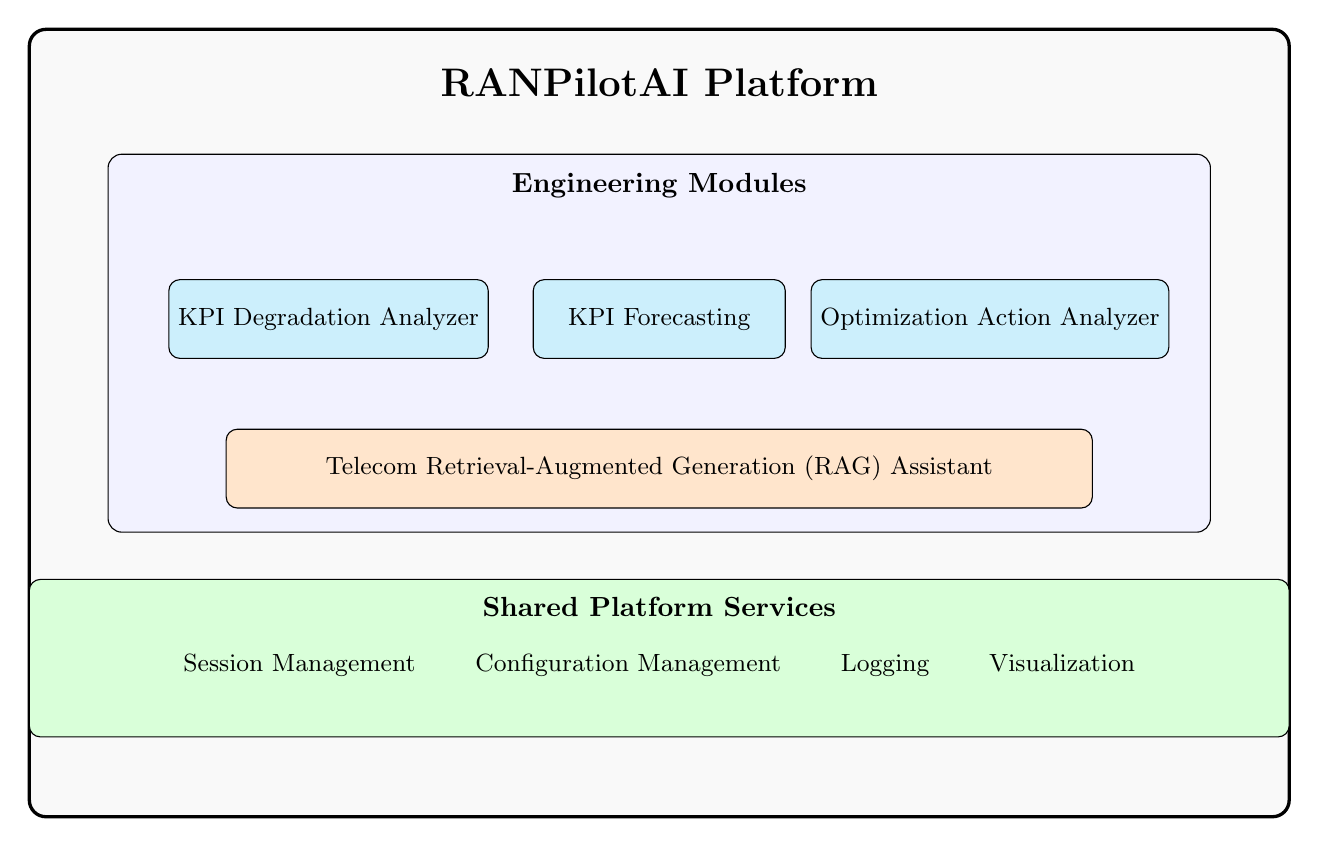
\begin{tikzpicture}[font=\small]

%%%%%%%%%%%%%%%%%%%%%%%%%%%%%%%%%%%%%%%%%%%%%%%%%%%%%%
% OUTER CONTAINER
%%%%%%%%%%%%%%%%%%%%%%%%%%%%%%%%%%%%%%%%%%%%%%%%%%%%%%

\node[
draw,
rounded corners=6pt,
very thick,
fill=gray!5,
minimum width=16cm,
minimum height=10cm,
anchor=north
] (platform) at (0,0)
{};

\node[font=\Large\bfseries]
at (platform.north)
[yshift=-0.7cm]
{RANPilotAI Platform};

%%%%%%%%%%%%%%%%%%%%%%%%%%%%%%%%%%%%%%%%%%%%%%%%%%%%%%
% ENGINEERING MODULES CONTAINER
%%%%%%%%%%%%%%%%%%%%%%%%%%%%%%%%%%%%%%%%%%%%%%%%%%%%%%

\node[
draw,
rounded corners=5pt,
fill=blue!5,
minimum width=14cm,
minimum height=4.8cm,
anchor=north
] (modules)
at ([yshift=-1.6cm]platform.north)
{};

\node[font=\bfseries]
at ([yshift=-0.4cm]modules.north)
{Engineering Modules};

%%%%%%%%%%%%%%%%%%%%%%%%%%%%%%%%%%%%%%%%%%%%%%%%%%%%%%
% KPI
%%%%%%%%%%%%%%%%%%%%%%%%%%%%%%%%%%%%%%%%%%%%%%%%%%%%%%

\node[
draw,
rounded corners,
fill=cyan!20,
minimum width=3.2cm,
minimum height=1cm
]
(kpi)
at ([xshift=-4.2cm,yshift=-2.1cm]modules.north)
{KPI Degradation Analyzer};

%%%%%%%%%%%%%%%%%%%%%%%%%%%%%%%%%%%%%%%%%%%%%%%%%%%%%%
% Forecast
%%%%%%%%%%%%%%%%%%%%%%%%%%%%%%%%%%%%%%%%%%%%%%%%%%%%%%

\node[
draw,
rounded corners,
fill=cyan!20,
minimum width=3.2cm,
minimum height=1cm
]
(forecast)
at ([xshift=0cm,yshift=-2.1cm]modules.north)
{KPI Forecasting};

%%%%%%%%%%%%%%%%%%%%%%%%%%%%%%%%%%%%%%%%%%%%%%%%%%%%%%
% Action
%%%%%%%%%%%%%%%%%%%%%%%%%%%%%%%%%%%%%%%%%%%%%%%%%%%%%%

\node[
draw,
rounded corners,
fill=cyan!20,
minimum width=3.2cm,
minimum height=1cm
]
(action)
at ([xshift=4.2cm,yshift=-2.1cm]modules.north)
{Optimization Action Analyzer};

%%%%%%%%%%%%%%%%%%%%%%%%%%%%%%%%%%%%%%%%%%%%%%%%%%%%%%
% RAG
%%%%%%%%%%%%%%%%%%%%%%%%%%%%%%%%%%%%%%%%%%%%%%%%%%%%%%

\node[
draw,
rounded corners,
fill=orange!20,
minimum width=11cm,
minimum height=1cm
]
(rag)
at ([yshift=-4cm]modules.north)
{Telecom Retrieval-Augmented Generation (RAG) Assistant};

%%%%%%%%%%%%%%%%%%%%%%%%%%%%%%%%%%%%%%%%%%%%%%%%%%%%%%
% SHARED SERVICES
%%%%%%%%%%%%%%%%%%%%%%%%%%%%%%%%%%%%%%%%%%%%%%%%%%%%%%

\node[
draw,
rounded corners,
fill=green!15,
minimum width=16cm,
minimum height=2cm,
anchor=north
]
(shared)
at ([yshift=-7cm]platform.north)
{};

\node[font=\bfseries]
at ([yshift=-0.35cm]shared.north)
{Shared Platform Services};

\node
at ([yshift=-1.1cm]shared.north)
{Session Management \qquad Configuration Management \qquad Logging \qquad Visualization};

\end{tikzpicture}

\caption{Overall architecture of the integrated RANPilotAI platform. The platform groups all analytical modules within a unified engineering environment while providing common platform services shared across the developed applications.}

\label{fig:platform_architecture}

\end{figure}

As illustrated in Figure~\ref{fig:platform_architecture}, the RANPilotAI platform is organized around two principal components. The first component contains the engineering modules responsible for implementing the intelligent analytical capabilities of the platform, whereas the second component provides the shared platform services required by all modules. This organization separates domain-specific processing from common software infrastructure, thereby improving maintainability and facilitating future extensions.

Each analytical module executes independently while sharing common services such as session management, configuration handling, logging, and visualization. Consequently, software duplication is minimized and a consistent user experience is maintained across the entire platform.
%%%%%%%%%%%%%%%%%%%%%%%%%%%%%%%%%%%%%%%%%%%%%%%%%%%%%%%%%%%%%%%%%%%%%%%%%%%%%%%%
\section{Integration Objectives}

The integration strategy adopted in the development of the RANPilotAI platform was guided by several software engineering objectives intended to improve the usability, maintainability, scalability, and extensibility of the system. Rather than focusing solely on integrating multiple analytical tools into a single application, the objective was to establish a modular software architecture capable of supporting future enhancements while maintaining a consistent engineering workflow.

The first objective was to provide a unified engineering environment that consolidates the complete RAN optimization workflow into a single platform. Instead of requiring engineers to execute separate applications for KPI analysis, forecasting, optimization planning, and standards consultation, all functionalities are accessible through the Telecom Hub.

The second objective was to maximize software modularity. Every analytical component was developed as an independent subsystem responsible for a specific engineering task. This separation of responsibilities minimizes software dependencies, simplifies debugging, and enables individual modules to evolve independently without affecting the remaining components.

Another important objective was the reuse of common software services. Instead of duplicating functionalities such as session management, configuration loading, logging, visualization, and navigation within every module, these services are centralized and shared across the entire platform. This approach reduces software complexity while improving maintainability and consistency.

Finally, the architecture was designed with extensibility as a primary consideration. Future analytical modules, artificial intelligence models, or optimization algorithms can be incorporated into the existing framework by integrating them into the Engineering Layer without requiring modifications to the overall platform architecture.

%%%%%%%%%%%%%%%%%%%%%%%%%%%%%%%%%%%%%%%%%%%%%%%%%%%%%%%%%%%%%%%%%%%%%%%%%%%%%%%%
\section{Layered Software Architecture}

From a software engineering perspective, the RANPilotAI platform follows a layered architecture that separates user interaction, application logic, engineering modules, and data management into distinct software layers. Such separation improves maintainability by ensuring that each layer is responsible for a well-defined set of functionalities while communicating only with adjacent layers.

Figure~\ref{fig:software_architecture} presents the layered software architecture adopted in the implementation of the platform.

%%%%%%%%%%%%%%%%%%%%%%%%%%%%%%%%%%%%%%%%%%%%%%%%%%%%%%%%%%%%%%%%%%%%%%%%%%%%%%%%

\begin{figure}[H]
\centering

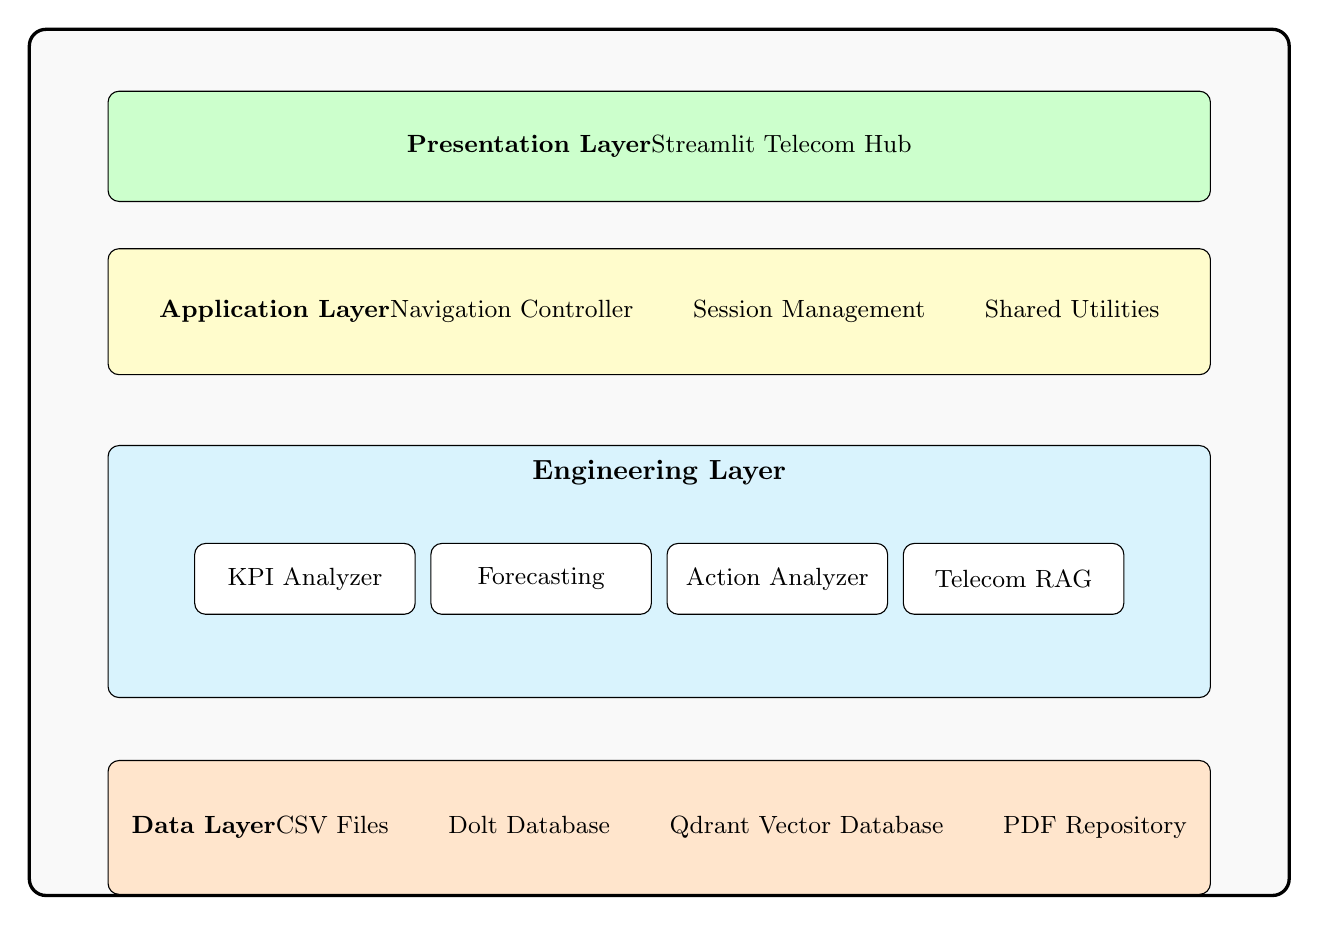
\begin{tikzpicture}[font=\small]

%%%%%%%%%%%%%%%%%%%%%%%%%%%%%%%%%%%%%%%%%%%%%%%%%%%%%%%%%%%%
% OUTER FRAME
%%%%%%%%%%%%%%%%%%%%%%%%%%%%%%%%%%%%%%%%%%%%%%%%%%%%%%%%%%%%

\node[
draw,
rounded corners=6pt,
very thick,
fill=gray!5,
minimum width=16cm,
minimum height=11cm
](frame){};

%%%%%%%%%%%%%%%%%%%%%%%%%%%%%%%%%%%%%%%%%%%%%%%%%%%%%%%%%%%%
% Presentation Layer
%%%%%%%%%%%%%%%%%%%%%%%%%%%%%%%%%%%%%%%%%%%%%%%%%%%%%%%%%%%%

\node[
draw,
rounded corners,
fill=green!20,
minimum width=14cm,
minimum height=1.4cm,
anchor=north
](presentation)
at ([yshift=-0.8cm]frame.north)
{\textbf{Presentation Layer}\\Streamlit Telecom Hub};

%%%%%%%%%%%%%%%%%%%%%%%%%%%%%%%%%%%%%%%%%%%%%%%%%%%%%%%%%%%%
% Application Layer
%%%%%%%%%%%%%%%%%%%%%%%%%%%%%%%%%%%%%%%%%%%%%%%%%%%%%%%%%%%%

\node[
draw,
rounded corners,
fill=yellow!20,
minimum width=14cm,
minimum height=1.6cm,
anchor=north
](application)
at ([yshift=-2.8cm]frame.north)
{\textbf{Application Layer}\\Navigation Controller \qquad Session Management \qquad Shared Utilities};

%%%%%%%%%%%%%%%%%%%%%%%%%%%%%%%%%%%%%%%%%%%%%%%%%%%%%%%%%%%%
% Engineering Layer
%%%%%%%%%%%%%%%%%%%%%%%%%%%%%%%%%%%%%%%%%%%%%%%%%%%%%%%%%%%%

\node[
draw,
rounded corners,
fill=cyan!15,
minimum width=14cm,
minimum height=3.2cm,
anchor=north
](engineering)
at ([yshift=-5.3cm]frame.north)
{};

\node[font=\bfseries]
at ([yshift=-0.35cm]engineering.north)
{Engineering Layer};

\node[
draw,
rounded corners,
fill=white,
minimum width=2.8cm,
minimum height=.9cm
]
at ([xshift=-4.5cm,yshift=-1.7cm]engineering.north)
{KPI Analyzer};

\node[
draw,
rounded corners,
fill=white,
minimum width=2.8cm,
minimum height=.9cm
]
at ([xshift=-1.5cm,yshift=-1.7cm]engineering.north)
{Forecasting};

\node[
draw,
rounded corners,
fill=white,
minimum width=2.8cm,
minimum height=.9cm
]
at ([xshift=1.5cm,yshift=-1.7cm]engineering.north)
{Action Analyzer};

\node[
draw,
rounded corners,
fill=white,
minimum width=2.8cm,
minimum height=.9cm
]
at ([xshift=4.5cm,yshift=-1.7cm]engineering.north)
{Telecom RAG};

%%%%%%%%%%%%%%%%%%%%%%%%%%%%%%%%%%%%%%%%%%%%%%%%%%%%%%%%%%%%
% Data Layer
%%%%%%%%%%%%%%%%%%%%%%%%%%%%%%%%%%%%%%%%%%%%%%%%%%%%%%%%%%%%

\node[
draw,
rounded corners,
fill=orange!20,
minimum width=14cm,
minimum height=1.7cm,
anchor=north
](data)
at ([yshift=-9.3cm]frame.north)
{\textbf{Data Layer}\\CSV Files \qquad Dolt Database \qquad Qdrant Vector Database \qquad PDF Repository};

\end{tikzpicture}

\caption{Layered software architecture of the RANPilotAI platform. The platform is organized into four logical layers separating presentation, application logic, engineering modules, and data management.}

\label{fig:software_architecture}

\end{figure}

The layered architecture shown in Figure~\ref{fig:software_architecture} separates the software into four logical layers, each responsible for a specific aspect of the platform. The Presentation Layer provides the graphical user interface through which engineers interact with the platform. The Application Layer manages navigation, user sessions, and shared software utilities that are reused across all analytical modules.

The Engineering Layer contains the four intelligent modules developed throughout this project. Each module executes independently while relying on the common services provided by the Application Layer. This separation ensures that modifications to one analytical component do not affect the remaining modules.

Finally, the Data Layer provides persistent storage and external resources required by the engineering modules. Structured datasets are maintained in CSV files, version-controlled engineering data are stored using Dolt, semantic document embeddings are managed by the Qdrant vector database, and the official 3GPP Technical Specifications are maintained within the PDF repository. This organization establishes a clear separation between data management and analytical processing while simplifying future maintenance and platform expansion.
%%%%%%%%%%%%%%%%%%%%%%%%%%%%%%%%%%%%%%%%%%%%%%%%%%%%%%%%%%%%%%%%%%%%%%%%%%%%%%%%
\section{Module Integration}

The RANPilotAI platform integrates four independent analytical modules into a unified engineering environment while preserving the autonomy of each subsystem. Rather than tightly coupling the modules, the integration strategy follows a modular design in which every component performs a dedicated engineering task and communicates with the Telecom Hub through standardized interfaces.

Each analytical module executes its own processing pipeline and maintains its own internal implementation. Consequently, modifications to one subsystem do not require changes to the remaining modules. This loose coupling improves software maintainability, facilitates debugging, and enables independent development of future platform extensions.

The KPI Degradation Analyzer is responsible for detecting abnormal network behaviour through KPI analysis. The KPI Forecasting module predicts future network performance using machine learning models. The Optimization Action Analyzer provides optimization recommendations based on historical engineering knowledge, while the Telecom Retrieval-Augmented Generation (RAG) Assistant enables engineers to interact with official 3GPP Technical Specifications using natural language.

Although these modules implement different analytical functionalities, they all follow the same execution model. Every request originates from the Telecom Hub, which identifies the requested service, forwards the request to the corresponding analytical module, receives the generated results, and presents them using a consistent graphical interface.

Figure~\ref{fig:module_interaction} illustrates the interaction between the Telecom Hub and the developed analytical modules.

%%%%%%%%%%%%%%%%%%%%%%%%%%%%%%%%%%%%%%%%%%%%%%%%%%%%%%%%%%%%%%%%%%%%%%%%%%%%%%%%

\begin{figure}[H]
\centering

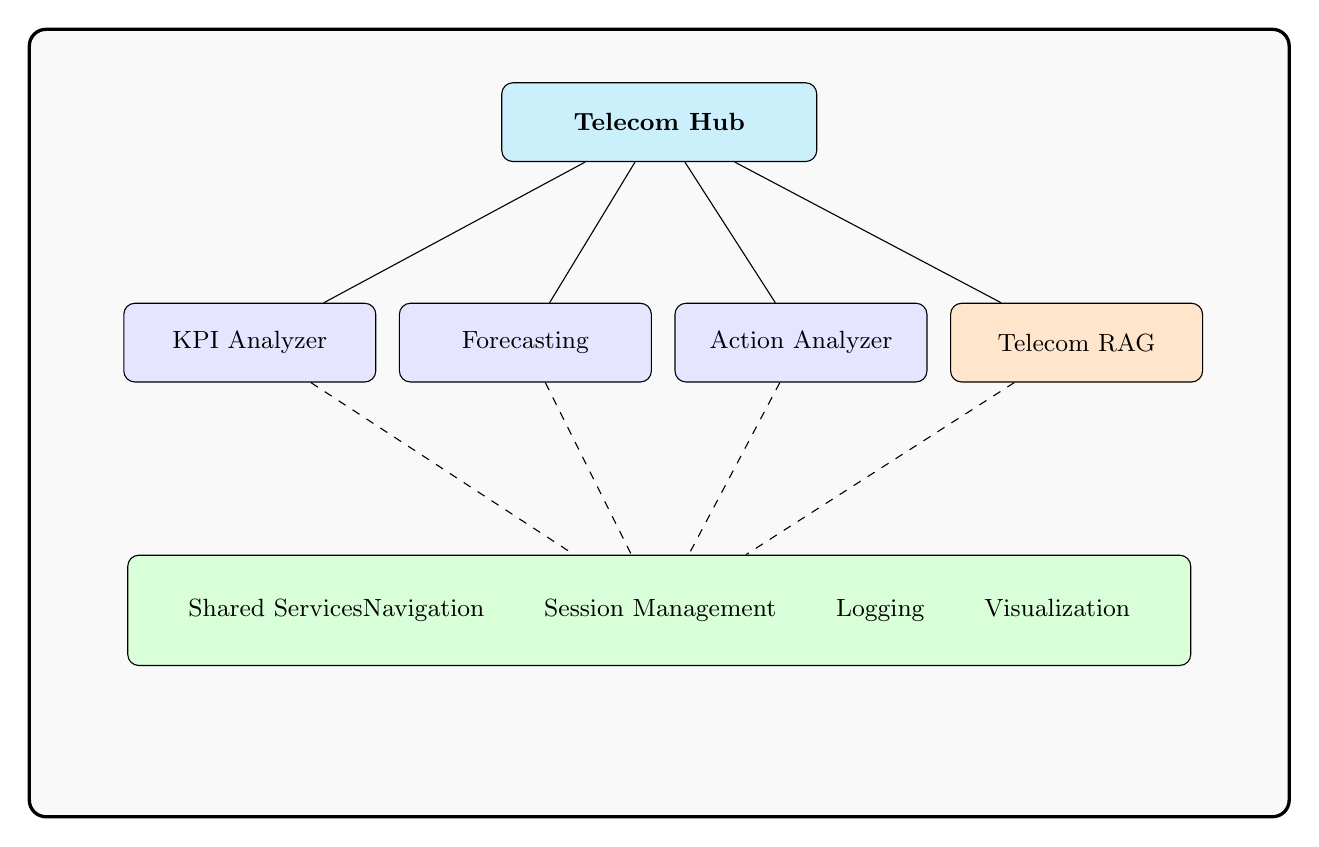
\begin{tikzpicture}[font=\small]

%%%%%%%%%%%%%%%%%%%%%%%%%%%%%%%%%%%%%%%%%%%%%%%%%%%%%%%%%%
% OUTER FRAME
%%%%%%%%%%%%%%%%%%%%%%%%%%%%%%%%%%%%%%%%%%%%%%%%%%%%%%%%%%

\node[
draw,
rounded corners=6pt,
very thick,
minimum width=16cm,
minimum height=10cm,
fill=gray!5
](frame){};

%%%%%%%%%%%%%%%%%%%%%%%%%%%%%%%%%%%%%%%%%%%%%%%%%%%%%%%%%%
% HUB
%%%%%%%%%%%%%%%%%%%%%%%%%%%%%%%%%%%%%%%%%%%%%%%%%%%%%%%%%%

\node[
draw,
rounded corners,
fill=cyan!20,
minimum width=4cm,
minimum height=1cm
](hub)
at ([yshift=-1.2cm]frame.north)
{\textbf{Telecom Hub}};

%%%%%%%%%%%%%%%%%%%%%%%%%%%%%%%%%%%%%%%%%%%%%%%%%%%%%%%%%%
% MODULES
%%%%%%%%%%%%%%%%%%%%%%%%%%%%%%%%%%%%%%%%%%%%%%%%%%%%%%%%%%

\node[
draw,
rounded corners,
fill=blue!10,
minimum width=3.2cm,
minimum height=1cm
](kpi)
at ([xshift=-5.2cm,yshift=-4cm]frame.north)
{KPI Analyzer};

\node[
draw,
rounded corners,
fill=blue!10,
minimum width=3.2cm,
minimum height=1cm
](forecast)
at ([xshift=-1.7cm,yshift=-4cm]frame.north)
{Forecasting};

\node[
draw,
rounded corners,
fill=blue!10,
minimum width=3.2cm,
minimum height=1cm
](action)
at ([xshift=1.8cm,yshift=-4cm]frame.north)
{Action Analyzer};

\node[
draw,
rounded corners,
fill=orange!20,
minimum width=3.2cm,
minimum height=1cm
](rag)
at ([xshift=5.3cm,yshift=-4cm]frame.north)
{Telecom RAG};

%%%%%%%%%%%%%%%%%%%%%%%%%%%%%%%%%%%%%%%%%%%%%%%%%%%%%%%%%%
% SHARED SERVICES
%%%%%%%%%%%%%%%%%%%%%%%%%%%%%%%%%%%%%%%%%%%%%%%%%%%%%%%%%%

\node[
draw,
rounded corners,
fill=green!15,
minimum width=13.5cm,
minimum height=1.4cm
](shared)
at ([yshift=-7.4cm]frame.north)
{Shared Services\\Navigation \qquad Session Management \qquad Logging \qquad Visualization};

%%%%%%%%%%%%%%%%%%%%%%%%%%%%%%%%%%%%%%%%%%%%%%%%%%%%%%%%%%
% CONNECTIONS
%%%%%%%%%%%%%%%%%%%%%%%%%%%%%%%%%%%%%%%%%%%%%%%%%%%%%%%%%%

\draw (hub)--(kpi);
\draw (hub)--(forecast);
\draw (hub)--(action);
\draw (hub)--(rag);

\draw[dashed](kpi)--(shared);
\draw[dashed](forecast)--(shared);
\draw[dashed](action)--(shared);
\draw[dashed](rag)--(shared);

\end{tikzpicture}

\caption{Module interaction within the RANPilotAI platform. The Telecom Hub coordinates user requests while common software services are shared among all analytical modules.}

\label{fig:module_interaction}

\end{figure}

As illustrated in Figure~\ref{fig:module_interaction}, all user requests are processed through the Telecom Hub before reaching the corresponding analytical module. This centralized coordination simplifies application navigation while preserving complete independence between the engineering subsystems.

The shared service layer provides reusable software functionality required by every module, including session management, application navigation, logging, and visualization. Consequently, common software components are implemented only once, reducing redundancy and improving maintainability.

%%%%%%%%%%%%%%%%%%%%%%%%%%%%%%%%%%%%%%%%%%%%%%%%%%%%%%%%%%%%%%%%%%%%%%%%%%%%%%%%
\section{Shared Components}

Although each analytical module implements a different engineering task, several software components are shared throughout the platform. Centralizing these functionalities simplifies software maintenance while ensuring a consistent user experience.

The principal shared components include:

\begin{itemize}

\item \textbf{Navigation Manager}

Responsible for routing users between the integrated analytical modules through the Telecom Hub.

\item \textbf{Session Manager}

Maintains user selections, application state, and module-specific parameters throughout the execution session.

\item \textbf{Configuration Manager}

Loads configuration files, model parameters, database connections, and application settings required by the analytical modules.

\item \textbf{Logging Service}

Records application events and execution information to simplify debugging and future maintenance.

\item \textbf{Visualization Engine}

Provides reusable plotting utilities and standardized graphical components that ensure consistent visualization across the platform.

\end{itemize}

Figure~\ref{fig:component_architecture} presents the logical organization of the shared software components.

%%%%%%%%%%%%%%%%%%%%%%%%%%%%%%%%%%%%%%%%%%%%%%%%%%%%%%%%%%%%%%%%%%%%%%%%%%%%%%%%
%%%%%%%%%%%%%%%%%%%%%%%%%%%%%%%%%%%%%%%%%%%%%%%%%%%%%%%%%%%%%%%%%%%%%%%%%%%%%%%%

\begin{figure}[H]
\centering

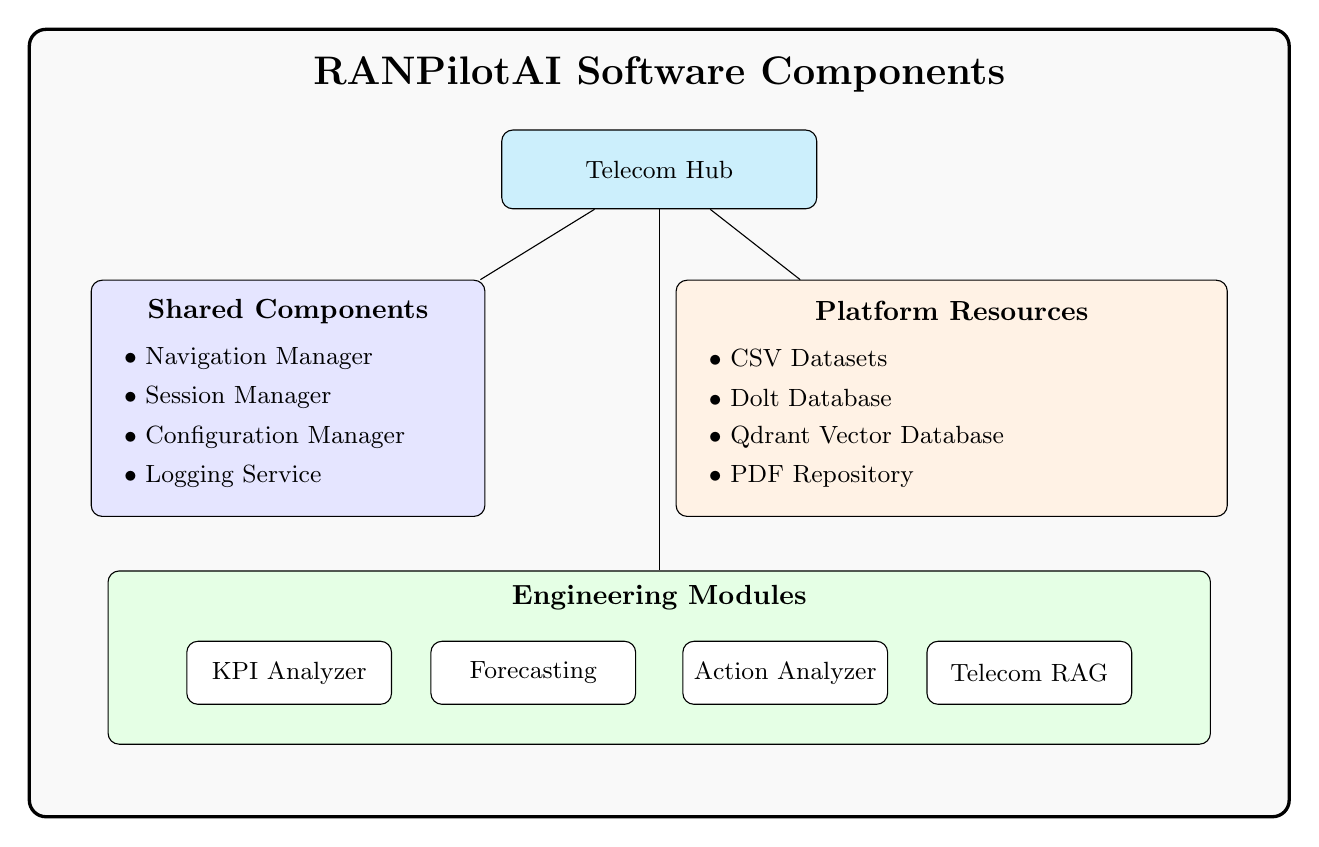
\begin{tikzpicture}[font=\small]

%%%%%%%%%%%%%%%%%%%%%%%%%%%%%%%%%%%%%%%%%%%%%%%%%%%%%%%%%%%%%%
% OUTER CONTAINER
%%%%%%%%%%%%%%%%%%%%%%%%%%%%%%%%%%%%%%%%%%%%%%%%%%%%%%%%%%%%%%

\node[
draw,
rounded corners=6pt,
very thick,
minimum width=16cm,
minimum height=10cm,
fill=gray!5
](system){};

\node[font=\bfseries\Large]
at ([yshift=-0.6cm]system.north)
{RANPilotAI Software Components};

%%%%%%%%%%%%%%%%%%%%%%%%%%%%%%%%%%%%%%%%%%%%%%%%%%%%%%%%%%%%%%
% TELECOM HUB
%%%%%%%%%%%%%%%%%%%%%%%%%%%%%%%%%%%%%%%%%%%%%%%%%%%%%%%%%%%%%%

\node[
draw,
rounded corners,
fill=cyan!20,
minimum width=4cm,
minimum height=1cm
](hub)
at ([yshift=-1.8cm]system.north)
{Telecom Hub};

%%%%%%%%%%%%%%%%%%%%%%%%%%%%%%%%%%%%%%%%%%%%%%%%%%%%%%%%%%%%%%
% LEFT COLUMN
%%%%%%%%%%%%%%%%%%%%%%%%%%%%%%%%%%%%%%%%%%%%%%%%%%%%%%%%%%%%%%

\node[
draw,
rounded corners,
fill=blue!10,
minimum width=5cm,
minimum height=3cm,
anchor=north west
](shared)
at ([xshift=0.8cm,yshift=-3.2cm]system.north west)
{};

\node[font=\bfseries]
at ([yshift=-0.4cm]shared.north)
{Shared Components};

\node[anchor=west]
at ([xshift=0.3cm,yshift=-1cm]shared.north west)
{$\bullet$ Navigation Manager};

\node[anchor=west]
at ([xshift=0.3cm,yshift=-1.5cm]shared.north west)
{$\bullet$ Session Manager};

\node[anchor=west]
at ([xshift=0.3cm,yshift=-2cm]shared.north west)
{$\bullet$ Configuration Manager};

\node[anchor=west]
at ([xshift=0.3cm,yshift=-2.5cm]shared.north west)
{$\bullet$ Logging Service};

%%%%%%%%%%%%%%%%%%%%%%%%%%%%%%%%%%%%%%%%%%%%%%%%%%%%%%%%%%%%%%
% RIGHT COLUMN
%%%%%%%%%%%%%%%%%%%%%%%%%%%%%%%%%%%%%%%%%%%%%%%%%%%%%%%%%%%%%%

\node[
draw,
rounded corners,
fill=orange!10,
minimum width=7cm,
minimum height=3cm,
anchor=north east
](resources)
at ([xshift=-0.8cm,yshift=-3.2cm]system.north east)
{};

\node[font=\bfseries]
at ([yshift=-0.4cm]resources.north)
{Platform Resources};

\node[anchor=west]
at ([xshift=0.3cm,yshift=-1cm]resources.north west)
{$\bullet$ CSV Datasets};

\node[anchor=west]
at ([xshift=0.3cm,yshift=-1.5cm]resources.north west)
{$\bullet$ Dolt Database};

\node[anchor=west]
at ([xshift=0.3cm,yshift=-2cm]resources.north west)
{$\bullet$ Qdrant Vector Database};

\node[anchor=west]
at ([xshift=0.3cm,yshift=-2.5cm]resources.north west)
{$\bullet$ PDF Repository};

%%%%%%%%%%%%%%%%%%%%%%%%%%%%%%%%%%%%%%%%%%%%%%%%%%%%%%%%%%%%%%
% ENGINEERING MODULES
%%%%%%%%%%%%%%%%%%%%%%%%%%%%%%%%%%%%%%%%%%%%%%%%%%%%%%%%%%%%%%

\node[
draw,
rounded corners,
fill=green!10,
minimum width=14cm,
minimum height=2.2cm
](modules)
at ([yshift=-8cm]system.north)
{};

\node[font=\bfseries]
at ([yshift=-0.35cm]modules.north)
{Engineering Modules};

\node[
draw,
rounded corners,
fill=white,
minimum width=2.6cm,
minimum height=.8cm
]
at ([xshift=-4.7cm,yshift=-1.3cm]modules.north)
{KPI Analyzer};

\node[
draw,
rounded corners,
fill=white,
minimum width=2.6cm,
minimum height=.8cm
]
at ([xshift=-1.6cm,yshift=-1.3cm]modules.north)
{Forecasting};

\node[
draw,
rounded corners,
fill=white,
minimum width=2.6cm,
minimum height=.8cm
]
at ([xshift=1.6cm,yshift=-1.3cm]modules.north)
{Action Analyzer};

\node[
draw,
rounded corners,
fill=white,
minimum width=2.6cm,
minimum height=.8cm
]
at ([xshift=4.7cm,yshift=-1.3cm]modules.north)
{Telecom RAG};

%%%%%%%%%%%%%%%%%%%%%%%%%%%%%%%%%%%%%%%%%%%%%%%%%%%%%%%%%%%%%%
% CONNECTIONS
%%%%%%%%%%%%%%%%%%%%%%%%%%%%%%%%%%%%%%%%%%%%%%%%%%%%%%%%%%%%%%

\draw (hub)--(shared);
\draw (hub)--(resources);
\draw (hub)--(modules);

\end{tikzpicture}

\caption{Component organization of the RANPilotAI platform showing the relationship between the Telecom Hub, shared software components, platform resources, and engineering modules.}

\label{fig:component_architecture}

\end{figure}

Figure~\ref{fig:component_architecture} illustrates the logical organization of the software components comprising the RANPilotAI platform. The Telecom Hub coordinates the interaction between users, shared software services, engineering modules, and platform resources. Shared components provide common functionality reused throughout the application, while the Engineering Modules implement the domain-specific analytical capabilities presented in the previous chapters.

Separating reusable software services from domain-specific modules significantly improves software maintainability by reducing duplication and establishing clear boundaries between infrastructure components and analytical functionality. Likewise, the explicit separation of platform resources enables individual modules to access common datasets, repositories, and vector databases without introducing unnecessary dependencies between the analytical subsystems.
%%%%%%%%%%%%%%%%%%%%%%%%%%%%%%%%%%%%%%%%%%%%%%%%%%%%%%%%%%%%%%%%%%%%%%%%%%%%%%%%
\section{Data Flow Between Modules}

The analytical modules integrated within the RANPilotAI platform exchange information through a centralized execution model coordinated by the Telecom Hub. Instead of allowing direct communication between individual modules, every user request is first processed by the Telecom Hub, which determines the selected analytical service and forwards the request to the corresponding processing engine. This centralized data flow simplifies software maintenance, reduces coupling between modules, and establishes a consistent execution model throughout the platform.

Although each analytical module implements a different processing pipeline, all modules follow the same execution sequence. User inputs are collected through the graphical interface, processed by the selected analytical engine, and finally returned to the Telecom Hub for visualization. Depending on the selected module, additional resources such as CSV datasets, the Dolt database, the Qdrant vector database, or the PDF repository may be accessed during execution.

Figure~\ref{fig:dataflow} illustrates the overall data flow within the RANPilotAI platform.

%%%%%%%%%%%%%%%%%%%%%%%%%%%%%%%%%%%%%%%%%%%%%%%%%%%%%%%%%%%%%%%%%%%%%%%%%%%%%%%%

\begin{figure}[H]
\centering

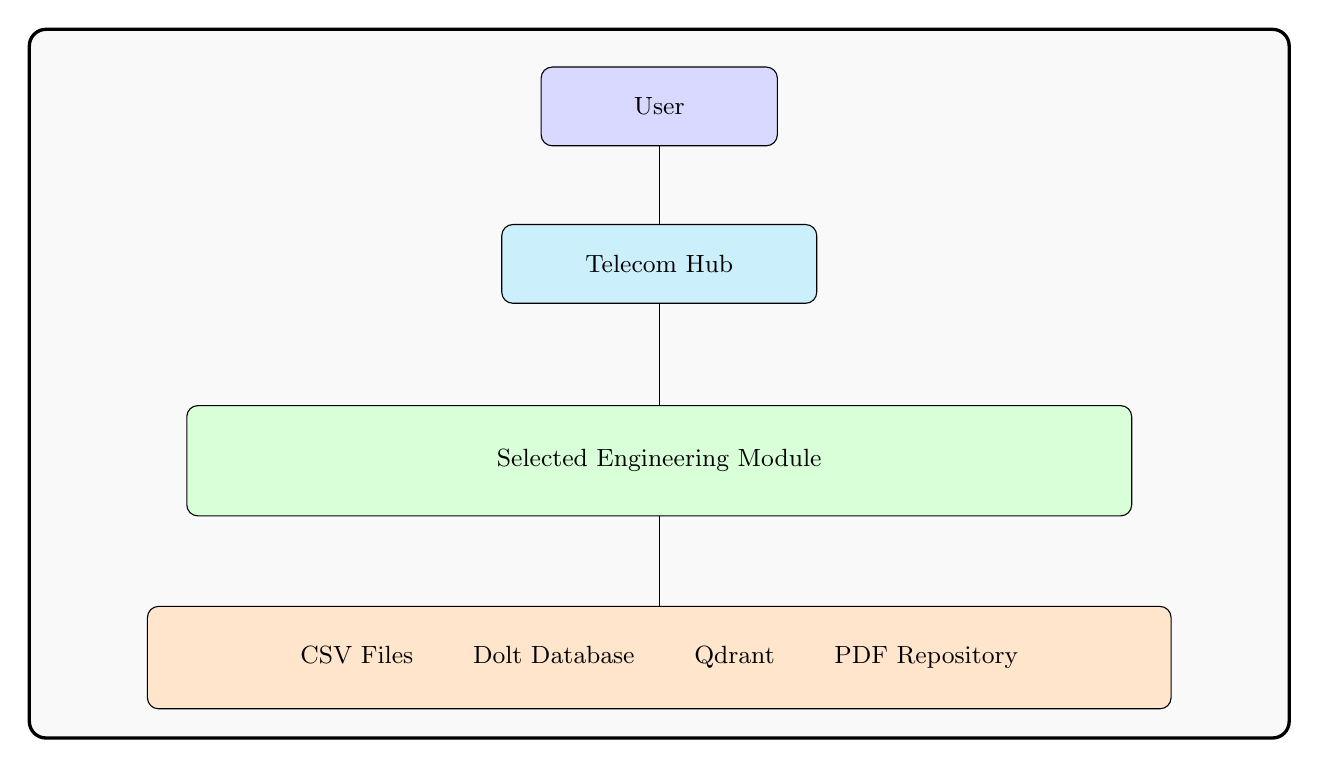
\begin{tikzpicture}[font=\small]

%%%%%%%%%%%%%%%%%%%%%%%%%%%%%%%%%%%%%%%%%%%%%%%%%%%%%%
% OUTER FRAME
%%%%%%%%%%%%%%%%%%%%%%%%%%%%%%%%%%%%%%%%%%%%%%%%%%%%%%

\node[
draw,
rounded corners=6pt,
minimum width=16cm,
minimum height=9cm,
fill=gray!5,
very thick
](frame){};

%%%%%%%%%%%%%%%%%%%%%%%%%%%%%%%%%%%%%%%%%%%%%%%%%%%%%%
% USER
%%%%%%%%%%%%%%%%%%%%%%%%%%%%%%%%%%%%%%%%%%%%%%%%%%%%%%

\node[
draw,
rounded corners,
fill=blue!15,
minimum width=3cm,
minimum height=1cm
](user)
at ([yshift=-1cm]frame.north)
{User};

%%%%%%%%%%%%%%%%%%%%%%%%%%%%%%%%%%%%%%%%%%%%%%%%%%%%%%
% HUB
%%%%%%%%%%%%%%%%%%%%%%%%%%%%%%%%%%%%%%%%%%%%%%%%%%%%%%

\node[
draw,
rounded corners,
fill=cyan!20,
minimum width=4cm,
minimum height=1cm
](hub)
at ([yshift=-3cm]frame.north)
{Telecom Hub};

%%%%%%%%%%%%%%%%%%%%%%%%%%%%%%%%%%%%%%%%%%%%%%%%%%%%%%
% ENGINE
%%%%%%%%%%%%%%%%%%%%%%%%%%%%%%%%%%%%%%%%%%%%%%%%%%%%%%

\node[
draw,
rounded corners,
fill=green!15,
minimum width=12cm,
minimum height=1.4cm
](engine)
at ([yshift=-5.5cm]frame.north)
{Selected Engineering Module};

%%%%%%%%%%%%%%%%%%%%%%%%%%%%%%%%%%%%%%%%%%%%%%%%%%%%%%
% DATA SOURCES
%%%%%%%%%%%%%%%%%%%%%%%%%%%%%%%%%%%%%%%%%%%%%%%%%%%%%%

\node[
draw,
rounded corners,
fill=orange!20,
minimum width=13cm,
minimum height=1.3cm
](data)
at ([yshift=-8cm]frame.north)
{CSV Files \qquad Dolt Database \qquad Qdrant \qquad PDF Repository};

%%%%%%%%%%%%%%%%%%%%%%%%%%%%%%%%%%%%%%%%%%%%%%%%%%%%%%
% LINES
%%%%%%%%%%%%%%%%%%%%%%%%%%%%%%%%%%%%%%%%%%%%%%%%%%%%%%

\draw (user)--(hub);

\draw (hub)--(engine);

\draw (engine)--(data);

\end{tikzpicture}

\caption{Overall data flow within the RANPilotAI platform. All requests are coordinated by the Telecom Hub before reaching the selected engineering module.}

\label{fig:dataflow}

\end{figure}

As shown in Figure~\ref{fig:dataflow}, the Telecom Hub acts as the intermediary between the user and the analytical modules. Every engineering request follows the same execution model regardless of the selected module. This unified data flow simplifies the software architecture and enables the platform to incorporate additional analytical modules without modifying the existing execution framework.

%%%%%%%%%%%%%%%%%%%%%%%%%%%%%%%%%%%%%%%%%%%%%%%%%%%%%%%%%%%%%%%%%%%%%%%%%%%%%%%%
\section{User Navigation Workflow}

The graphical user interface of RANPilotAI was designed to provide a simple and intuitive navigation experience. Rather than exposing the internal complexity of the analytical modules, users interact only with the Telecom Hub, which presents all available engineering tools through a unified interface.

Figure~\ref{fig:activity} illustrates the workflow followed by a typical user during interaction with the platform.

%%%%%%%%%%%%%%%%%%%%%%%%%%%%%%%%%%%%%%%%%%%%%%%%%%%%%%%%%%%%%%%%%%%%%%%%%%%%%%%%

\begin{figure}[H]
\centering

\begin{tikzpicture}[font=\small,node distance=1.3cm]

\node[draw,ellipse,fill=green!20](start){Start};

\node[process,below=of start]
(open)
{Open RANPilotAI};

\node[process,below=of open]
(select)
{Select Module};

\node[decision,below=of select]
(decision)
{Module?};

\node[process,left=3cm of decision]
(kpi)
{Run KPI Analysis};

\node[process,right=3cm of decision]
(rag)
{Ask Engineering Question};

\node[process,below=2cm of decision]
(result)
{Display Results};

\node[draw,ellipse,fill=red!15,below=of result]
(end)
{End};

\draw[->](start)--(open);

\draw[->](open)--(select);

\draw[->](select)--(decision);

\draw[->](decision)--node[above]{KPI}(kpi);

\draw[->](decision)--node[above]{RAG}(rag);

\draw[->](kpi)--(result);

\draw[->](rag)--(result);

\draw[->](result)--(end);

\end{tikzpicture}

\caption{Typical user navigation workflow within the RANPilotAI platform.}

\label{fig:activity}

\end{figure}

The workflow begins when the user launches the platform and selects one of the available analytical modules. The Telecom Hub then forwards the request to the selected subsystem, waits for the analytical results, and presents them through the graphical interface. This interaction model remains identical regardless of the selected engineering module, thereby ensuring a consistent user experience throughout the platform.

%%%%%%%%%%%%%%%%%%%%%%%%%%%%%%%%%%%%%%%%%%%%%%%%%%%%%%%%%%%%%%%%%%%%%%%%%%%

%%%%%%%%%%%%%%%%%%%%%%%%%%%%%%%%%%%%%%%%%%%%%%%%%%%%%%%%%%%%%%%%%%%%%%%%%%%%%%%%
\section{Deployment Environment}

The RANPilotAI platform was designed as a lightweight web-based application that can be deployed on a single workstation without requiring a distributed computing infrastructure. The deployment strategy prioritizes simplicity, portability, and ease of installation while providing sufficient computational resources for the analytical tasks implemented throughout the platform.

The Streamlit framework serves as the presentation layer of the application, providing an interactive graphical user interface through which users access the different engineering modules. Since Streamlit executes as a local web application, users can interact with the platform through a standard web browser without installing additional client software.

All engineering modules execute within the same Python runtime environment. This unified execution model simplifies dependency management, facilitates communication between modules, and enables the reuse of common software components. Furthermore, executing the analytical modules locally reduces network latency and allows the platform to remain operational even in environments with limited Internet connectivity.

The platform relies on several local data resources. Structured engineering datasets are maintained as CSV files, historical engineering information is managed using the Dolt database, semantic document embeddings are stored within the Qdrant vector database, and official 3GPP Technical Specifications are maintained locally as PDF documents. These resources collectively provide the information required by the different analytical modules while remaining independent from external services.

External communication is required only during the execution of the Telecom Retrieval-Augmented Generation (RAG) Assistant. Once relevant engineering information has been retrieved from the local vector database, the generated prompt is forwarded to a Large Language Model (LLM) through the OpenRouter API to produce the final engineering response. Consequently, the majority of platform operations remain local while external communication is limited to natural language generation.

This deployment strategy provides an effective balance between computational efficiency and intelligent reasoning capabilities. Local execution ensures rapid analytical processing and secure management of engineering datasets, whereas cloud-based language models provide advanced natural language understanding without increasing the complexity of the local deployment.

%%%%%%%%%%%%%%%%%%%%%%%%%%%%%%%%%%%%%%%%%%%%%%%%%%%%%%%%%%%%%%%%%%%%%%%%%%%%%%%%
\section{Platform Scalability}

Scalability was considered as one of the principal design objectives during the development of the RANPilotAI platform. Rather than implementing a monolithic software application, the platform adopts a modular architecture in which every analytical component operates as an independent subsystem connected through the Telecom Hub.

This modular organization enables future engineering modules to be incorporated without modifying the existing analytical components. New machine learning models, optimization algorithms, or AI assistants can be integrated by implementing the required processing logic and registering the module within the Telecom Hub navigation framework.

The shared software infrastructure further improves scalability by centralizing common functionalities such as session management, configuration loading, logging, visualization, and application routing. Since these services are reused by all analytical modules, the integration of additional functionalities does not introduce unnecessary software duplication.

The platform architecture also supports future migration toward distributed deployment environments. Although the current implementation executes on a single workstation, the modular software organization allows individual analytical modules to be deployed independently as web services or containerized applications. Such an architecture would enable computational workloads to be distributed across multiple processing nodes while preserving the unified user experience provided by the Telecom Hub.

Finally, the data management layer was designed to accommodate continuous expansion. Additional engineering datasets, telecommunications standards, optimization knowledge bases, and vector collections can be incorporated without requiring structural modifications to the software architecture. This capability ensures that the platform can evolve alongside future mobile communication technologies and emerging artificial intelligence techniques.

%%%%%%%%%%%%%%%%%%%%%%%%%%%%%%%%%%%%%%%%%%%%%%%%%%%%%%%%%%%%%%%%%%%%%%%%%%%%%%%%
\section{Integration Challenges}

The integration of multiple analytical modules into a unified engineering platform introduced several software engineering challenges throughout the development process. Although each module was developed independently, integrating them into a single application required careful architectural decisions to ensure consistency, maintainability, and reliable execution.

One of the primary challenges involved coordinating heterogeneous analytical components. The developed modules employ different computational approaches, including traditional machine learning models, time-series forecasting algorithms, retrieval-based information systems, and Large Language Models. Establishing a unified execution model capable of supporting these diverse computational paradigms required the implementation of a common interaction framework through the Telecom Hub.

Another challenge concerned software dependency management. Since each analytical module relies on specialized Python libraries and external packages, maintaining compatibility between software components required careful version management and standardized project organization. Consolidating all dependencies into a common execution environment significantly simplified deployment while reducing software conflicts.

Maintaining a consistent graphical user interface also represented an important engineering consideration. Despite the diversity of analytical tasks performed by the individual modules, users should experience a unified interaction model throughout the platform. Standardizing visualization components, navigation mechanisms, and application layouts therefore became an essential aspect of the integration strategy.

Managing local and external resources presented an additional challenge. While most analytical operations rely exclusively on locally available datasets and vector databases, the Telecom RAG Assistant communicates with external language models through the OpenRouter API. Coordinating local retrieval with cloud-based response generation required careful management of network communication while preserving application responsiveness.

Finally, ensuring extensibility without sacrificing maintainability influenced many architectural decisions throughout the project. The adoption of modular software components, reusable utilities, and standardized interfaces enables future platform expansion while minimizing the impact of modifications on the existing system.
%%%%%%%%%%%%%%%%%%%%%%%%%%%%%%%%%%%%%%%%%%%%%%%%%%%%%%%%%%%%%%%%%%%%%%%%%%%%%%%%
\section{Future Extensions}

Although the current implementation of the RANPilotAI platform provides a comprehensive intelligent environment for Radio Access Network (RAN) optimization, its modular software architecture enables several opportunities for future enhancement. The separation between the analytical modules and the Telecom Hub allows new functionalities to be incorporated without significant architectural modifications, ensuring that the platform can evolve alongside future telecommunications technologies.

One potential extension involves the integration of real-time network monitoring capabilities. Instead of relying solely on offline engineering datasets, future versions of the platform could establish direct communication with Operations Support Systems (OSS) or Network Management Systems (NMS) to analyze live network measurements. Such integration would enable continuous KPI monitoring and provide engineers with immediate analytical feedback based on current network conditions.

Another promising enhancement concerns the deployment architecture. Although the current implementation executes on a single workstation, the platform can be migrated to a cloud-native environment using containerization technologies such as Docker and orchestration platforms such as Kubernetes. This deployment model would improve scalability, simplify software maintenance, and enable concurrent access by multiple engineers.

The analytical capabilities of the platform can also be expanded by incorporating additional machine learning and artificial intelligence models. Future versions may include anomaly detection algorithms, reinforcement learning techniques for automatic optimization, predictive maintenance models, and advanced traffic forecasting approaches. Since each analytical component operates independently, these capabilities can be integrated while preserving the existing software architecture.

The Telecom Retrieval-Augmented Generation (RAG) Assistant can also be enhanced by integrating domain-specific language models trained exclusively on telecommunications literature and vendor documentation. Such models would improve the accuracy of technical responses and provide more specialized engineering recommendations. Furthermore, expanding the document repository to include vendor-specific implementation guides, operational manuals, and optimization procedures would significantly increase the knowledge available to the assistant.

Finally, future versions of RANPilotAI may provide collaborative engineering capabilities through multi-user authentication, centralized project management, shared engineering workspaces, and automated report generation. These features would transform the platform from an individual engineering assistant into a collaborative decision-support system capable of supporting larger operational teams.

%%%%%%%%%%%%%%%%%%%%%%%%%%%%%%%%%%%%%%%%%%%%%%%%%%%%%%%%%%%%%%%%%%%%%%%%%%%%%%%%
\section{Chapter Summary}

This chapter presented the system integration strategy adopted during the development of the RANPilotAI platform. Unlike the previous chapters, which focused on the implementation of individual analytical modules, this chapter described how these independent components were combined into a unified engineering environment capable of supporting multiple Radio Access Network optimization tasks.

The chapter introduced the overall platform architecture, the layered software organization, the interaction between analytical modules, and the shared software components that provide common functionality across the platform. Furthermore, the deployment environment, scalability considerations, and software engineering challenges encountered during system integration were discussed in detail.

The modular architecture adopted throughout the development process establishes a flexible and extensible software foundation that simplifies future platform evolution while maintaining a consistent user experience. By integrating machine learning models, Retrieval-Augmented Generation techniques, optimization algorithms, and engineering knowledge within a single software environment, RANPilotAI provides a comprehensive intelligent platform for supporting modern Radio Access Network optimization activities.

The following chapter presents the overall conclusions of this work, summarizes the principal contributions of the project, and outlines potential directions for future research and development.
